\documentclass[12pt]{article}
\usepackage[papersize={8.5in,11in}, margin = 1in]{geometry}
\usepackage[utf8]{inputenc}
\usepackage{setspace}
\usepackage{amssymb}
\usepackage{amsmath}
\usepackage{physics}
\usepackage{fancyhdr}
\usepackage{enumitem}
\usepackage{lastpage}
\usepackage[none]{hyphenat}%%%%
\usepackage[scr]{rsfso}
\usepackage[dvipsnames]{xcolor}
\usepackage{graphicx}
\usepackage{caption}
\captionsetup{font=footnotesize}
\usepackage{subcaption}
\usepackage{float}
\usepackage{listings}
\usepackage{titlesec}
\usepackage{algorithm}
\usepackage{algpseudocode}
\usepackage{placeins}
\usepackage{newtxtext,newtxmath}
\usepackage{ragged2e}
\usepackage{url}
\bibliographystyle{unsrt}

\titleformat{\section}[block]{\normalfont\Large\bfseries}{\thesection}{1em}{}
\titlespacing{\section}{0pt}{*1.5}{0pt}
\titlespacing{\subsection}{0pt}{*0.75}{0pt}

\usepackage{hyperref}
\hypersetup{
    colorlinks=true,
    linktoc=all,
    linkcolor=teal,
    urlcolor=teal,
    citecolor=teal,
}
\graphicspath{{pics/}}

% because khushant's title page is wonky -BA
\usepackage{atbegshi}% http://ctan.org/pkg/atbegshi
% \AtBeginDocument{\AtBeginShipoutNext{\AtBeginShipoutDiscard}}

% for codeblocks
\definecolor{codegreen}{rgb}{0,0.6,0}
\definecolor{codegray}{rgb}{0.5,0.5,0.5}
\definecolor{codepurple}{rgb}{0.58,0,0.82}
\definecolor{backcolour}{rgb}{0.95,0.95,0.92}

\lstdefinestyle{mystyle}{
    backgroundcolor=\color{backcolour},   
    commentstyle=\color{codegreen},
    keywordstyle=\color{magenta},
    numberstyle=\tiny\color{codegray},
    stringstyle=\color{codepurple},
    basicstyle=\ttfamily\footnotesize,
    breakatwhitespace=false,         
    breaklines=true,                 
    captionpos=b,                    
    keepspaces=true,                 
    numbers=left,                    
    numbersep=5pt,                  
    showspaces=false,                
    showstringspaces=false,
    showtabs=false,                  
    tabsize=2
}

\lstset{style=mystyle}

\pagestyle{fancy}
\fancyhead[L]{\small University of Pennsylvania \\ MEAM 6240 - Distributed Robotics}
\fancyhead[R]{\small Benjamin Aziel and Jason Chen \\ \today}
\fancyfoot[C]{Page \thepage\ of \pageref{LastPage}} 
\fancyfoot[C]{Page \thepage \hspace{1pt} of \pageref{LastPage}}

\newcommand{\Volume}{{\ooalign{\hfil$V$\hfil\cr\kern0.08em--\hfil\cr}}}
\begin{document}

% https://www.lifewire.com/text-alignment-tips-1074943
% i'm very biased towards flushleft. sorry justify fans

\thispagestyle{empty}
\newcommand{\titleName}{Performance Analysis of the Boids Algorithm in Coverage Scenarios\\[.4cm]
\textmd{\LARGE MEAM 6240 - Distributed Robotics}}
\begin{titlepage} 
	\newcommand{\HRule}{\rule{\linewidth}{0.5mm}}
	\center
	\textsc{\LARGE University of Pennsylvania}\\[2.5cm] 
	{\color{black} \HRule\\[0.4cm]}
	{\huge\bfseries \titleName}\\[0.4cm] 
	{\color{black} \HRule\\[0.4cm]}
	\begin{minipage}{0.4\textwidth}
		\begin{flushleft}
			\large
			\textit{Authors:}\\
            \textsc{Benjamin Aziel} \\
            \textsc{Jason Chen}\\
            \text{ }\\
		\end{flushleft}
	\end{minipage}
	~
	\begin{minipage}{0.4\textwidth}
		\begin{flushright}
			\large
			\textit{Professor:}\\
			\textsc{Cynthia Sung}\\ 
            \text{ }\\
            \text{ }\\
		\end{flushright}
	\end{minipage}
	\vfill

    \vfill
	{\large Last Updated: \today}
	\vfill
%----------------------------------------------------------------------------------------
\end{titlepage}

\fancypagestyle{tocstyle}{
    \fancyhf{} 
    \renewcommand{\footrulewidth}{0pt} 
    \renewcommand{\headrulewidth}{0.4pt} 
}

\thispagestyle{tocstyle}
\tableofcontents
\pagenumbering{gobble}
\pagebreak

\abovedisplayskip=6pt
\belowdisplayskip=0pt
\abovedisplayshortskip=0pt
\belowdisplayshortskip=0pt

\pagenumbering{arabic}
\setcounter{page}{1}

\setlength{\parindent}{0pt}
\setlength{\parskip}{0.5em}
\section*{Abstract}

The objective of this project is to implement and analyze the boids model for flocking behavior, with a focus on optimizing its effectiveness for coverage tasks through systematic tuning of key behavioral parameters. By adjusting the core gains that govern alignment, cohesion, and separation, the same underlying framework can yield a wide spectrum of emergent group dynamics, ranging from tight, cohesive flocking to deliberate spatial dispersion. The implementation explores the practical applications of these behaviors for distributed robotics systems, with quantitative analysis of exploration across various parameter configurations and environmental scenarios.

\newpage

\section{Introduction}

Collective behavior is a well-documented phenomenon in natural systems, observable in bird flocks, fish schools, and herds of terrestrial animals. These systems exhibit coordinated, large-scale movement patterns that appear to emerge from simple local interactions between individuals. Craig Reynolds formalized this concept with the boids model in his 1986 paper ``\emph{Flocks, Herds, and Schools: A Distributed Behavior Model}'' \cite{reynolds1987flocks}. This project builds on that framework by reimplementing Reynolds' original algorithm and extending it for use in robotic exploration tasks, with a focus on performance optimization through parameter tuning.

The boids model operates on three fundamental steering rules, as seen in Figure \ref{fig:force_diagram}:
\begin{itemize}[nosep]
    \item \textbf{Separation}: Avoid collisions with nearby agents
    \item \textbf{Alignment}: Match velocity and direction with neighbors
    \item \textbf{Cohesion}: Move towards the average position of local flockmates
\end{itemize}

\begin{figure}[h!]
    \centering
    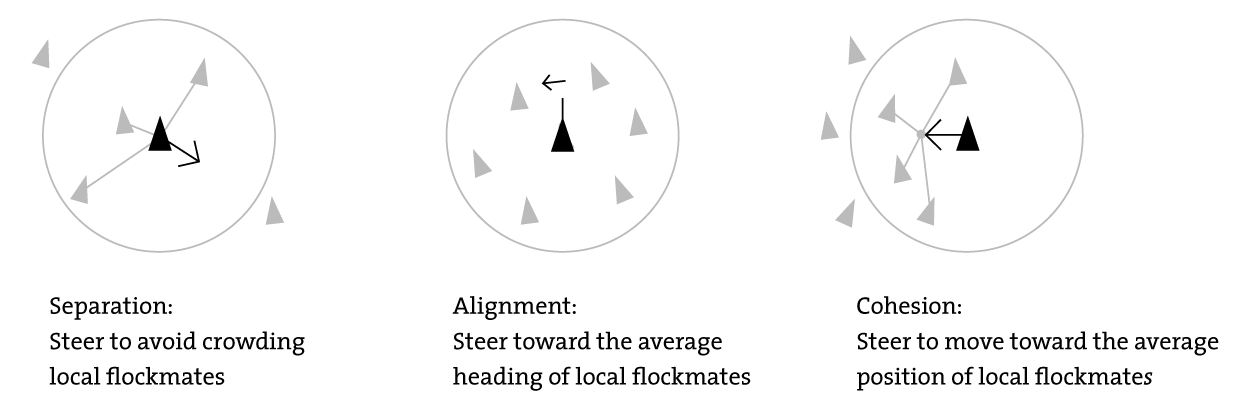
\includegraphics[width=0.7\linewidth]{force_diagram.png}
    \caption{Illustration of local force computations for a single boid \(i\). Cohesion pulls the agent toward neighbors, alignment encourages matching velocity, and separation pushes the agent away from close agents. Obstacle and wall avoidance forces are repulsive and operate independently. Source: \cite{martinez2023boids}}
    \label{fig:force_diagram}
  \end{figure}

Despite their simplicity, these rules give rise to complex, decentralized group dynamics without any global coordination. This makes the model highly relevant to applications such as swarm robotics, where systems must be scalable, robust to individual failures, and capable of adapting to unknown or dynamic environments.

In this work, the boids model is repurposed for robotic coverage. Rather than merely replicating natural flocking behavior, the focus is on optimizing behavioral parameters, i.e., the weightings of separation, alignment, and cohesion, to achieve task-oriented objectives. The goal is to maximize coverage efficiency, defined by metrics such as area coverage and dispersion uniformity.

The simulator used for optimization also includes options for real-time parameter adjustment and obstacle avoidance capabilities. Systematic experimentation across the gain space enables identification of configurations that strike a balance between coordinated movement and spatial dispersion to allow for more effective coverage.

\section{Simulation Framework}

To support systematic exploration and parameter optimization, a custom boids-based simulator was developed using PyGame, a Python library for 2D graphics and user interaction. The simulator can be seen in Figure \ref{fig:boids_sim}. This platform enables real-time visualization, modular integration of behavioral components, and controlled experimentation under various environmental conditions. The simulation runs at a fixed timestep of 60 frames per second, ensuring consistent physics and predictable agent behavior across different hardware configurations. The system uses discrete-time Euler integration to update each boid's velocity and position per frame. This ensures predictable physical updates and consistent motion behavior.

\begin{figure}[h!]
    \centering
    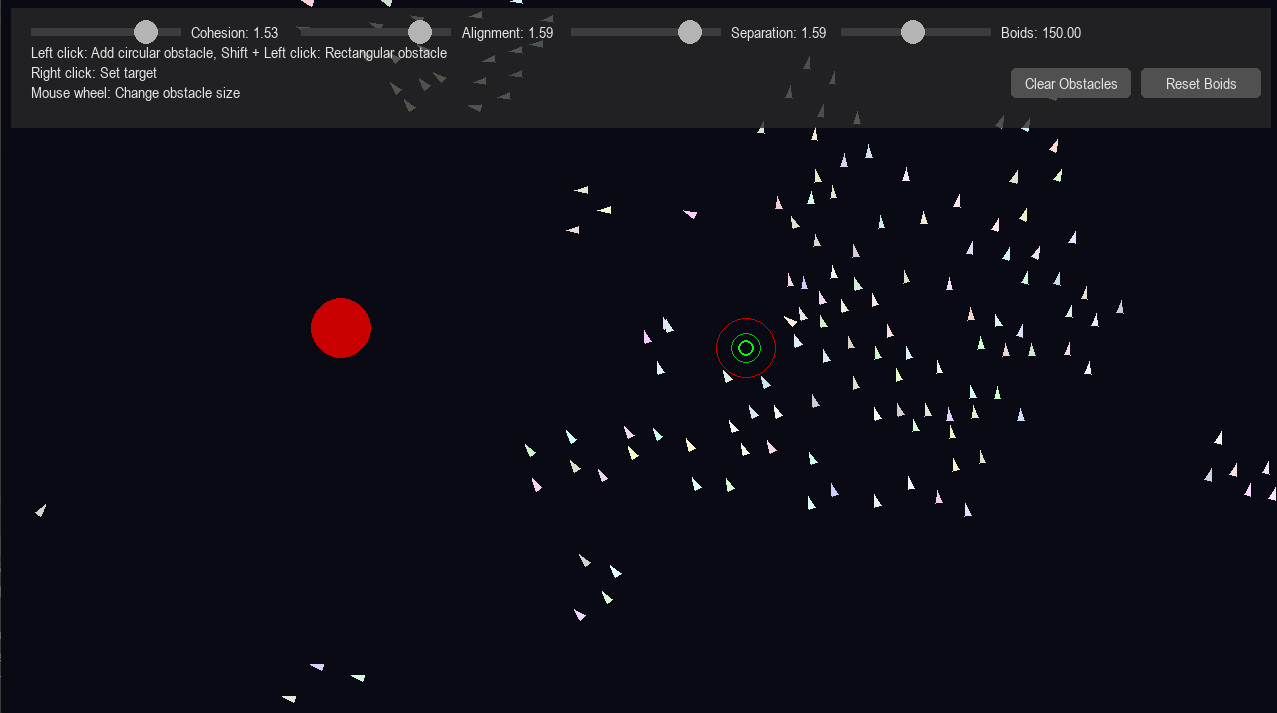
\includegraphics[width=0.7\linewidth]{boids_sim.png}
    \caption{Interactive simulation of the Boids model during runtime. A red circle indicates a user-placed obstacle, while the green target marker represents the global goal toward which boids are directed. The UI at the top enables real-time adjustment of behavioral gains for cohesion, alignment, and separation, as well as boid count and obstacle management.}
    \label{fig:boids_sim}
  \end{figure}

The architecture is modular, with the following components:
\begin{itemize}[nosep]
    \item \texttt{boid}, which implements the \texttt{Boid} class with core flocking behaviors
    \item \texttt{obstacles}, which defines obstacle representations and collision management
    \item \texttt{ui}, which handles rendering and interactive controls
    \item \texttt{simulation}, which coordinates all system components and updates
    \item \texttt{main}, which initializes the boids and launches the simulation
\end{itemize}

The simulator implements the three canonical behaviors central to the boids model: separation, alignment, and cohesion. Each of these arises from decentralized interaction rules, in which agents make steering decisions based on local sensing. Specifically, each boid perceives only other agents within a fixed perception radius and within a field-of-view cone, mimicking limited sensing capabilities found in physical agents.

The mathematical model implemented in this work is adapted from the original Boids formulation by Reynolds~\cite{reynolds1987flocks} and formalized based on principles presented in the Distributed Robotics course notes by Sung~\cite{sung2025distributed}. Within its perceived neighborhood \(\mathcal{N}_i(t)\), boid \(i\) computes a set of behavioral forces that determine its instantaneous acceleration. Let \(x_i \in \mathbb{R}^2\) denote the position of boid \(i\), and \(\dot{x}_i \in \mathbb{R}^2\) its velocity at time \(t\). These quantities are used to define the core behavioral forces governing flocking.

The collision avoidance force \(f_{\text{col}}\) pushes the agent away from nearby flockmates to reduce local density. It is computed as a repulsive sum of displacement vectors from all neighbors in the visible neighborhood, scaled by a gain \(k_{\text{col}}\):
\[ f_\text{col} = k_\text{col} \sum_{j \in \mathcal{N}_i(t)} (x_i - x_j) \]

For alignment and cohesion, the vector sum is normalized by the number of neighbors to compute the local average velocity and position, respectively; this ensures that the resulting steering direction reflects the group's overall tendency rather than being biased by the number or density of nearby agents. The alignment force \(f_\text{ali}\) encourages velocity matching with nearby flockmates. It is defined as the difference between the average velocity of visible neighbors and the agent’s current velocity, scaled by a gain \(k_\text{ali}\): 
\[ f_\text{ali} = k_\text{ali} \left( \frac{1}{|\mathcal{N}_i(t)|} \sum_{j \in \mathcal{N}_i(t)} \dot{x}_j - \dot{x}_i \right) \]

The cohesion force \(f_\text{coh}\) attracts the agent toward the center of mass of its neighborhood. It is computed as the displacement from the agent to the average position of its neighbors, scaled by \(k_\text{coh}\): 
\[ f_\text{coh} = k_\text{coh} \left( \frac{1}{|\mathcal{N}_i(t)|} \sum_{j \in \mathcal{N}_i(t)} x_j - x_i \right) \]

In addition to these flocking behaviors, agents also respond to environmental geometry. The obstacle avoidance force \(f_{\text{obs}}\) is computed as a sum of repulsive vectors from nearby obstacle locations \(o_m\), scaled by inverse squared distance to produce a smooth avoidance behavior. A small constant \(\varepsilon > 0\) is added to the denominator to avoid singularities:
\[ f_\text{obs} = \sum_m \frac{x_i - o_m}{\left( \|x_i - o_m\| + \varepsilon \right)^2} \]

A special case of this is the wall repulsion force \(f_\text{wall}\), which keeps agents within the rectangular simulation bounds. This is treated as implicit obstacle repulsion from the domain boundaries of width \(W\) and height \(H\): \[ f_\text{wall} = k_\text{wall} \begin{bmatrix}
\frac{1}{x_i + \varepsilon} - \frac{1}{W - x_i + \varepsilon} \\
\frac{1}{y_i + \varepsilon} - \frac{1}{H - y_i + \varepsilon}
\end{bmatrix} \]

The simulator also supports direct user interaction to dynamically configure the environment during runtime. Users can place obstacles in the environment using mouse input. The simulator currently supports both circular and rectangular obstacle types. This system enables the creation of realistic and heterogeneous test environments without modifying source code. When the user clicks in the PyGame simulation window while in obstacle-placement mode, a new obstacle is instantiated at the cursor location and added to the environment. This mechanism allows rapid prototyping of complex environments, such as cluttered indoor scenes, facilitating evaluation of the flock's navigational agility and adaptability under different spatial constraints.

In addition to environmental modification, the simulator includes a targeting mechanism that enables the user to assign a global heading objective to the flock. When enabled, a target point (typically set via mouse click) is rendered on the simulation display. Each boid will then attempt to steer towards this point using a dedicated target-seeking behavior.

\sloppypar
To realistically simulate physical constraints, a prioritized acceleration framework was implemented. Each boid has a limited total acceleration budget per timestep. When multiple behavioral directives are active, higher-priority behaviors consume available acceleration first. Lower-priority behaviors are only applied if residual capacity remains. The prioritization hierarchy is as follows, from highest to lowest:

\[\text{Obstacle Avoidance} > \text{Separation} > \text{Alignment} > \text{Cohesion} > \text{Target Seeking}\]

Each force is applied sequentially and scaled to fit within the remaining acceleration budget. If the magnitude of a force exceeds the available capacity, it is truncated proportionally. Once the budget is depleted, all subsequent forces in the priority list are skipped for that timestep. This leads to behavior that dynamically adapts to situational demands, closely resembling real-world decision making under physical constraints. Compared to traditional weighted vector summation, this method provides a more biologically plausible and computationally realistic behavior model.

\section{Coverage Task and Optimization}

To evaluate the utility of the boids model for distributed exploration, a coverage task was defined in which agents aim to maximize the percentage of a 2D environment they collectively traverse. The objective is to identify gain configurations (specifically the cohesion, alignment, and separation gains) that optimize coverage while preserving desirable collective behaviors such as dispersion, obstacle negotiation, and responsiveness.

\subsection{Task Definition and Environments}

Three distinct environments, as shown in Figure \ref{fig:boids_maps} were developed to assess the generality of exploration performance across varying spatial constraints:
\begin{itemize}[nosep]
    \item \textbf{Empty Map}: An unobstructed arena used as a baseline for evaluating pure flocking behavior and maximum dispersion potential
    \item \textbf{Narrow Corridor}: A scenario containing a bottleneck, requiring agents to transition through a constrained passage, thereby testing local reformation and dispersion under topological stress
    \item \textbf{Cafeteria Map}: A cluttered layout composed of circular (tables) and square (chairs) obstacles arranged in a semi-structured environment, simulating realistic indoor navigation challenges
\end{itemize}

\begin{figure}[h!]
    \centering
    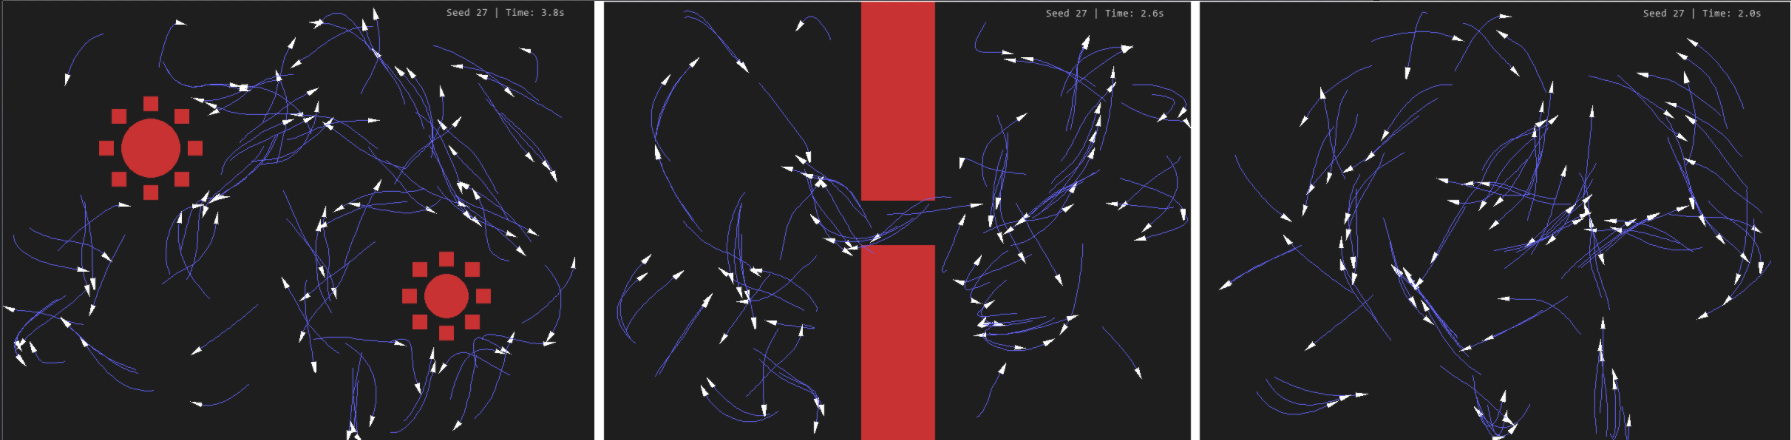
\includegraphics[width=\linewidth]{boids_maps.png}
    \caption{Evaluation environments used for testing: cafeteria map, narrow corridor, and empty map, from left to right. Each layout presents different navigational challenges and constraints.}
    \label{fig:boids_maps}
  \end{figure}

\subsection{Coverage Metrics}

The coverage percentage is defined:
\[\text{Coverage} = \frac{\text{Unique visited pixels}}{\text{Total traversable pixels}} \times 100\%\]

Here, traversable pixels are defined as all non-obstacle pixels in the environment. A pixel is considered visited if it falls within a fixed-radius disk centered at a boid's position during any simulation frame. Specifically, each boid marks pixels within a radius of 2 pixels per frame, representing an approximation of the physical footprint of the agent. Only pixels outside of obstacle regions are counted as visited.

Additionally, a spatial distribution visualization (coverage heatmap) encodes visitation frequency via color intensity. This provides insight into patterns of redundancy, area neglect, and localized over-exploration. Heatmaps support qualitative assessment of whether agents are uniformly distributing coverage effort.

\subsection{Simulation Details}

Compared to the interactive PyGame-based simulation used for development and visualization, the batch evaluation simulation used for optimization is a stripped-down and performance-focused variant. This version preserves the core behavioral logic but removes all non-essential components to maximize computational efficiency and scalability.

The most notable change is the complete removal of graphics and visualization routines. Unlike the interactive simulation, which runs within a PyGame window and provides real-time visual feedback, the optimization version runs entirely headless. No rendering, frame drawing, or event handling is performed. This allows for simulations to be executed in parallel using the \texttt{multiprocessing} module, significantly accelerating the parameter search. Each simulation job is defined as a unique pair of a sampled gain vector and a fixed random seed. These jobs are distributed across worker processes to evaluate parameter configurations in parallel, significantly reducing overall runtime.

Additionally, user interaction capabilities are stripped away. The optimization simulation does not support real-time obstacle placement or target assignment. Instead, each environment is instantiated procedurally at the start of each trial using one of the three aforementioned predefined layouts.

Real-time parameter adjustment via sliders is replaced with randomized sampling of gain vectors within predefined bounds. Each gain vector is evaluated in a self-contained trial, allowing for fully automated search over the parameter space.

Each trial begins by instantiating \(N = 100\) boids, each with randomized initial positions and velocities. Initial velocities are oriented uniformly at random in \([0, 2\pi)\) radians and scaled by the maximum speed. A validation step ensures that no boid is initialized within an obstacle's geometry. Each simulation runs for a fixed duration of 60 seconds, and the system updates at 60 frames per second, totaling 3600 simulation steps per trial. At each frame, behavioral forces are computed for each boid according to the prioritized behavior stack, the boids' states are updated, and visited pixel maps are updated accordingly.

In the optimization code, the simulation domain is adjusted into an 800\(\times\)600 pixel grid. This reduced resolution was chosen to balance coverage fidelity with computational efficiency, allowing for faster execution of large numbers of parallel trials without compromising the spatial complexity of the environment.

All environmental features and agent initializations are fully deterministic given a fixed random seed, ensuring repeatable and unbiased performance measurements. For each gain vector, the simulation is evaluated across three random seeds (27, 729, and 4913). These seeds are used to initialize the PRNG for placement, velocity, and repeated sampling if the initial sample was rejected due to obstacle conflict.

\subsection{Optimization Process}

\sloppypar
A systematic random search procedure was employed to identify high-performing behavior parameters. A total of 2000 gain vectors were randomly sampled within the defined bounds, and other parameters like maximum acceleration, obstacle avoidance gain, and FOV were fixed. For each gain vector, simulations were run in parallel across all three random seeds using multiprocessing, and the results were aggregated. The output of each run includes per-seed coverage and the average across seeds. The best-performing parameter vector for each environment was identified by sorting configurations by average coverage percentage.

\section{Results and Discussion}

\emph{Preliminary Results (04/24):}

The parameter sweep over the cohesion \(k_\text{coh}\), alignment \(k_\text{ali}\), and separation \(k_\text{col}\) gains was conducted in the Cafeteria environment, which contains a densely cluttered layout of circular and rectangular obstacles. Results (average coverage \% vs. each gain individually) are shown in Figure \ref{fig:gains}.

\begin{figure}[h!]
\centering
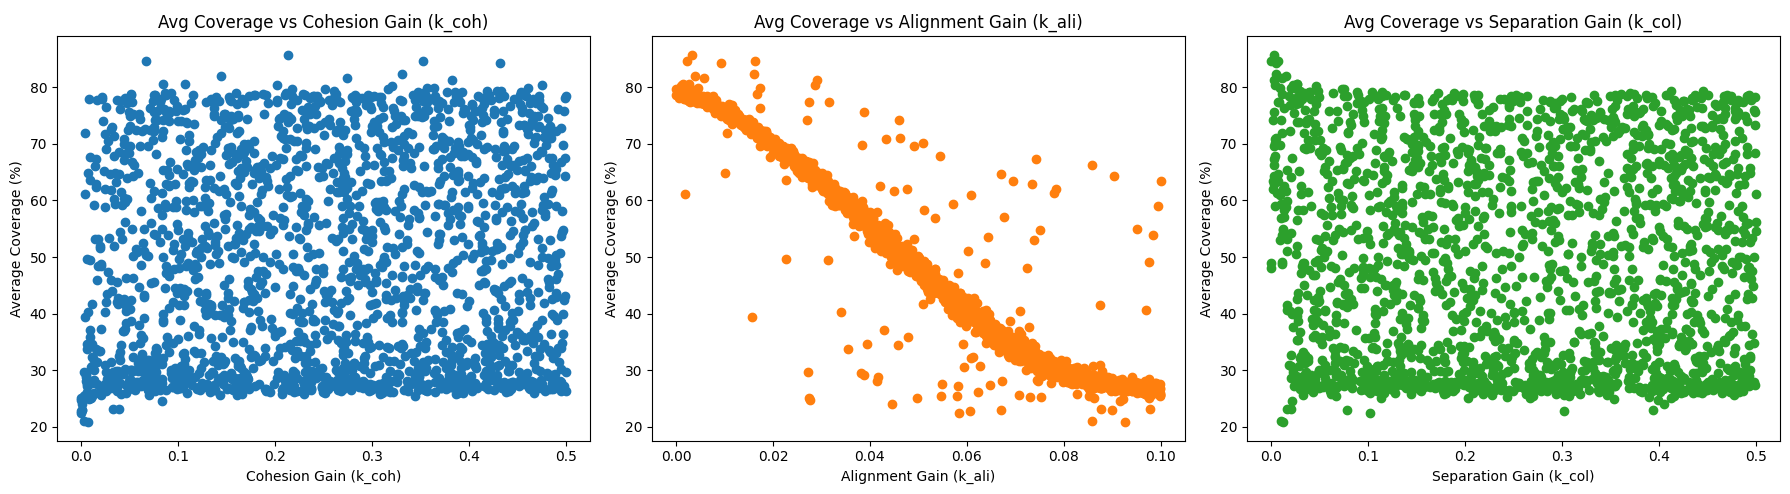
\includegraphics[width=\linewidth]{gains.png}
\caption{Coverage scores across sampled gain vectors in the parameter search.}
\label{fig:gains}
\end{figure}

Coverage does not appear to be highly sensitive to the value of \(k_\text{coh}\) within the sampled range \([0.0, 0.5]\). While some of the highest-performing configurations occur at mid-range cohesion values, there is no clear trend, suggesting that cohesion plays a secondary role in coverage performance under heavy obstacle density. There is a clear negative correlation between alignment gain \(k_\text{ali}\) and coverage. This indicates that excessive alignment behavior degrades exploration quality, likely due to overcoordination among boids. In highly constrained environments like the Cafeteria map, maintaining a unified velocity vector reduces group dispersion and leads to redundant coverage of already-visited areas. Finally, the relationship between separation gain \(k_\text{col}\) and coverage is quantitatively similar to cohesion: relatively flat with no dominant trend. However, slightly high coverage densities are observed for configurations with \(k_\text{col} > 0.2\), indicating that maintaining interpersonal distance modestly contributes to dispersion and therefore broader coverage. This effect is less pronounced than with alignment but still suggests some sensitivity to the balance between repulsion and aggregation.

The highest-performing parameter configuration observed in the Cafeteria environment achieved an average coverage of 85.76\%. Coverage over time can be analyzed in Figure \ref{fig:caf_cov}, and frequency of coverage can be analyzed in Figure \ref{fig:caf_heatmap}. This occurred at gain vector \((k_\text{coh}, k_\text{ali}, k_\text{col}) = (0.213, 0.003, 0.003)\), which supports the hypothesis that minimizing coordinated velocity (alignment) while maintaining a moderate degree of spatial structure (via cohesion and separation) yields the most effective exploratory behavior. 

On the heatmaps, warmer colors indicate higher visit frequency. The overlaid blue outlines denote obstacle locations, including circular tables and surrounding square chairs. Despite stochastic initialization, all runs show high overall coverage, with slight variations in path redundancy and unvisited regions.

\begin{figure}[h!]
    \centering
    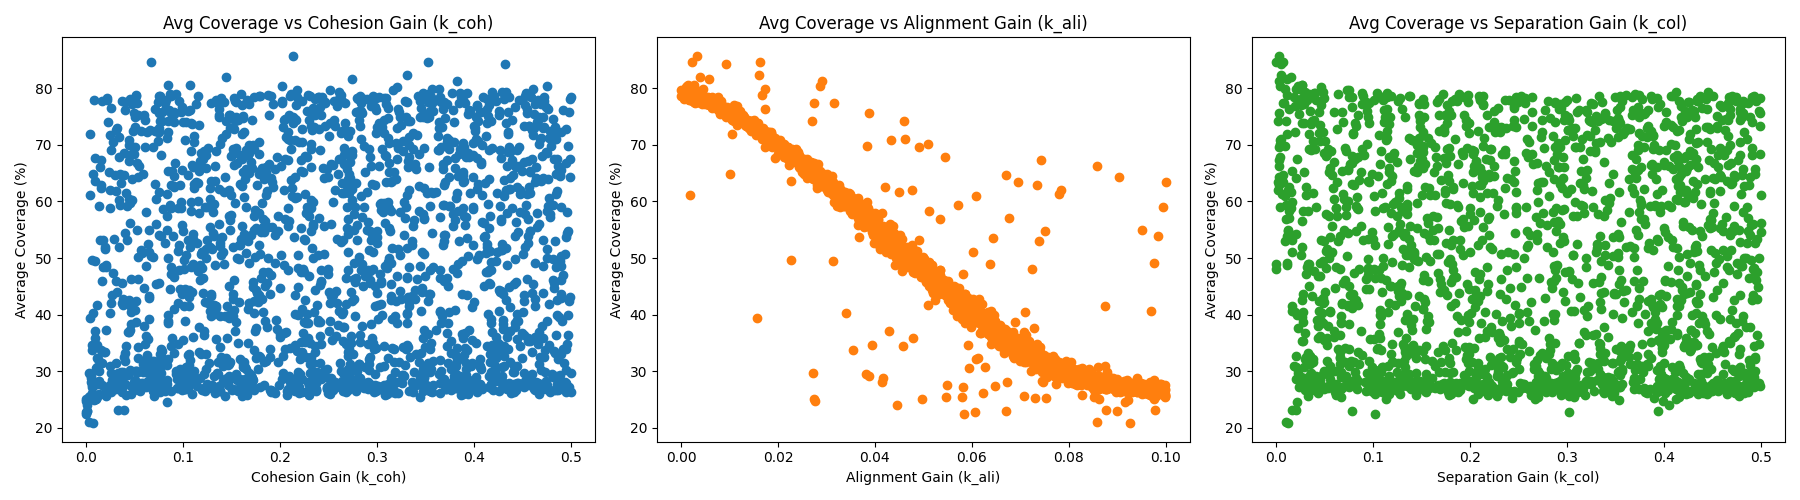
\includegraphics[width=\linewidth]{cov_vs_gains/cafeteria_100.png}
    \caption{Line plots showing percent coverage over time for optimal gain vector, for three seeds.}
    \label{fig:caf_cov}
  \end{figure}

\begin{figure}[h!]
\centering
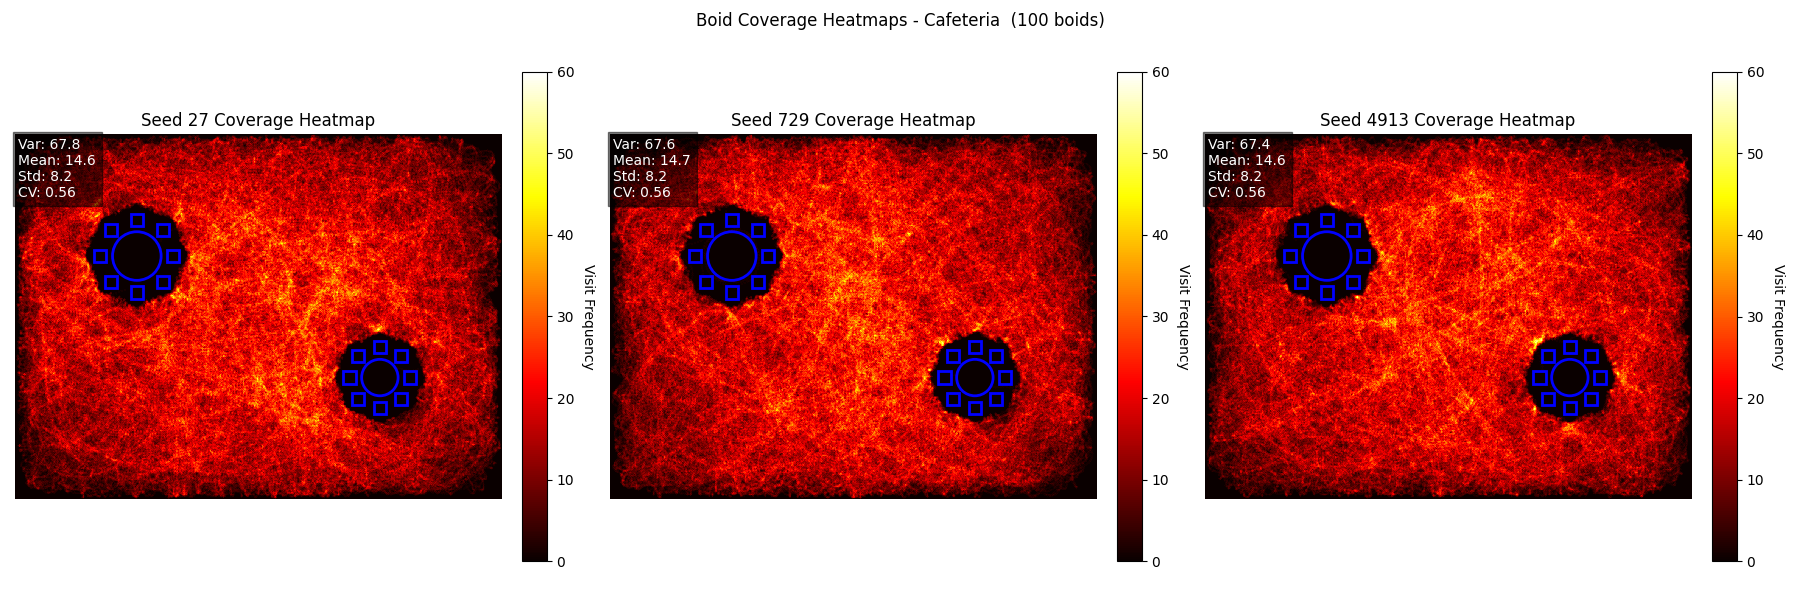
\includegraphics[width=\linewidth]{heatmaps/cafeteria_100.png}
\caption{Coverage heatmaps for the Cafeteria environment using three different random seeds (27, 729, and 4913).}
\label{fig:caf_heatmap}
\end{figure}

These findings suggest that for coverage tasks in cluttered environments, heterogeneity in agent motion is more beneficial than tight flocking. Coordination behaviors that promote uniformity, e.g., alignment, should be downregulated, while decentralized repulsion and loose cohesion provide a useful trade-off between safety and spatial dispersion. These design principles align well with real-world swarm robotics, where diversity in motion paths is key to avoiding stagnation and ensuring high coverage efficiency.

\section{Limitations and Future Work}

\sloppypar
While the simulation successfully demonstrates how optimized boids parameters can enhance exploration performance, it operates under several simplifying assumptions that constrain generalizability. The model assumes perfect sensing, with agents having full and accurate awareness of all neighbors within a fixed perception radius and field of view. In practice, sensor noise, occlusions, and limited sensing fidelity can disrupt coordination and reduce system robustness. Additionally, all agents are modeled as homogeneous, with identical sensing, speed, and actuation capabilities. This assumption simplifies implementation but overlooks the influence of heterogeneous agent capabilities, which are common in real robotic systems and can have meaningful effects on group dynamics.

The environment is modeled as static and fully known, with obstacles placed at initialization and held fixed throughout the simulation. In contrast, many practical exploration tasks take place in dynamic and uncertain environments where obstacles may move or appear unpredictably. The simulation also omits physical considerations such as friction, inertia, or energy consumption. These factors are critical for deployment on real platforms, particularly when operating in domains like aerial or underwater robotics, where control authority is limited and energy management is a major constraint.

\section{Conclusion}

This study demonstrates that the boids model, when tuned appropriately, can serve as a viable decentralized framework for distributed coverage tasks in complex environments. By systematically optimizing the core behavioral parameters governing alignment, cohesion, and separation, significant improvements in exploration efficiency were achieved, particularly in cluttered scenarios where coordination must be balanced with dispersion. The results suggest that minimal alignment, coupled with arbitrary cohesion and separation, yields the most effective coverage behavior under spatial constraints. These insights support the broader applicability of bio-inspired swarm algorithms in real-world robotic systems, particularly in scenarios where scalability, robustness, and adaptability are critical.

\bibliography{references}

\appendix

\end{document}
